\documentclass[12pt, notitlepage]{article}
\usepackage[utf8]{inputenc}
\usepackage{multicol}
\usepackage{multirow}
\usepackage[margin=0.5in]{geometry}
\usepackage[utf8]{inputenc}
\usepackage{tikz}
\usepackage{graphicx}
\graphicspath{{./images/}}
\usepackage{soul}
\usepackage{listings}
\usepackage{xcolor}
\usetikzlibrary{arrows}
\usepackage{mathtools}
\usepackage{amsmath}
\usepackage{pgfplots}
\pgfplotsset{compat=1.8}
\usepgfplotslibrary{statistics}
\usepackage{float}
\usepackage{tabto}
\usepackage{caption}

\title{CSE 145 - Homework 2}
\author{Daniel Xiong (dxiong5@ucsc.edu)}
\date{Due May 14}

\begin{document}
\maketitle
\section{Introduction}
The goal of this project was to data mine the \texttt{Customer\_Churn.xlsx} dataset, which contains 20,000 entries with 12 variables describing features of customers of a mobile phone provider. We aimed to predict the variable \texttt{"LEAVE"}, which represented whether a given customer would stay or leave the company. To achieve this goal, we first create some visualizations to try and understand the data. We then used the K-Means algorithm to cluster the data to further analyze the properties of the data. Finally, we chose predictive models to predict whether or not a customer would stay or leave the company.

\section{Tools Used}
This assignment was completed using Python 3.7 (scikit-learn $>=$ 0.22.1, pandas, matplotlib).

\section{Data Understanding}
One important metric is information gain, which is a measure of how much an attribute improves entropy over the whole segmentation it creates. In the context of supervised segmentation, information gain measures the knowledge gained by splitting the set on all values of a single attribute. \textbf{Figure 1} is a bar graph that ranks the information gain of all the attributes in decreasing order, with \texttt{"HOUSE"} being the attribute with the greatest information gain value.\\\\
write about next visualization\\\\
The code for these visualizations can be found in \texttt{visualizations.py}. 
\begin{figure}[H]
	\centering
	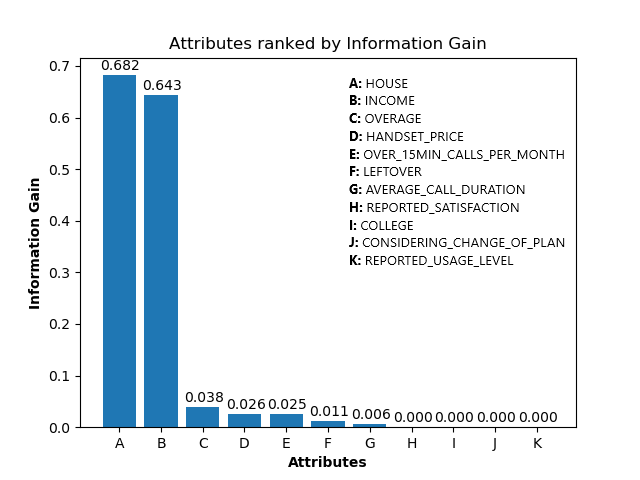
\includegraphics[scale=0.8]{InformationGain.png}
	\caption{Attributes ranked by their information gain}
\end{figure}
\begin{figure}[H]
	\centering 
	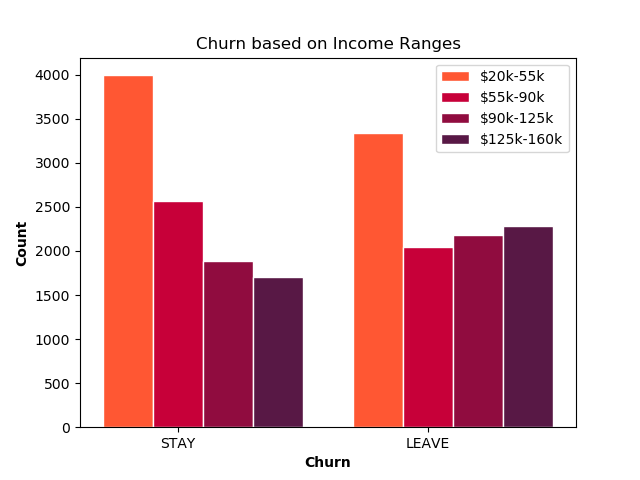
\includegraphics[scale=0.8]{IncomeVsChurn.png}
\end{figure}

\section{Customer Segmentation with K-Means}
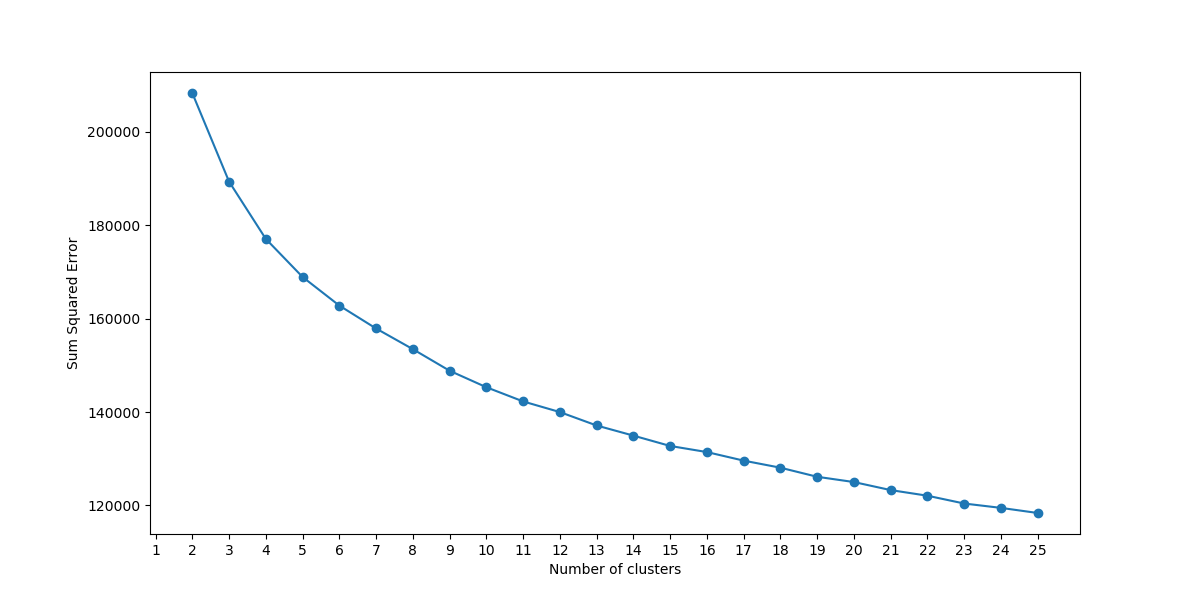
\includegraphics[scale=0.6]{kmeans_SSE.png}\\
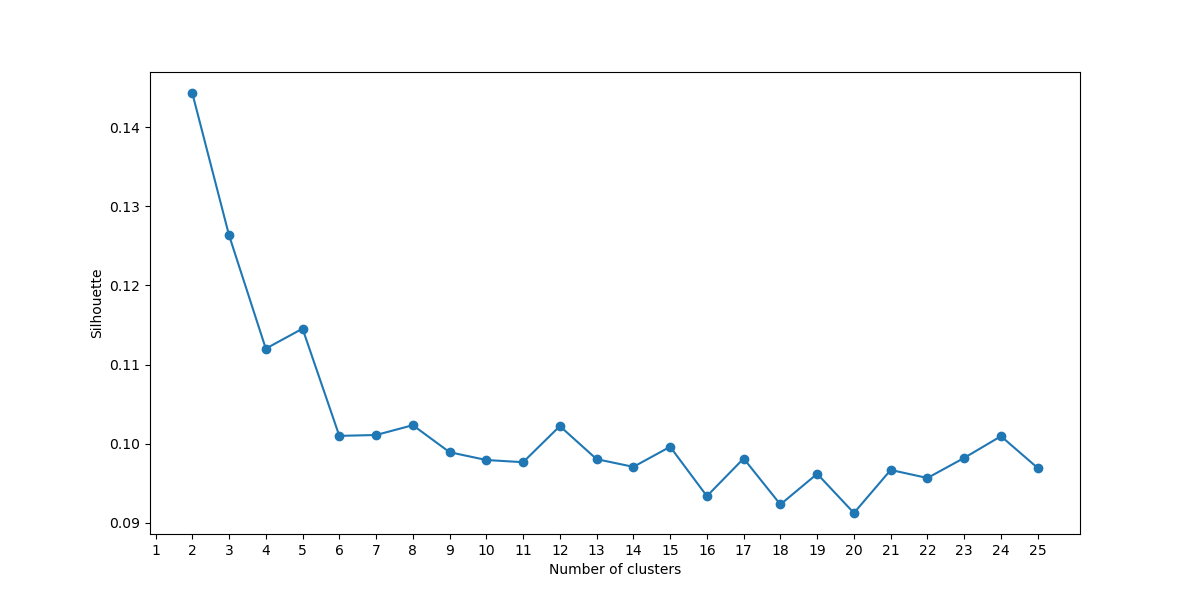
\includegraphics[scale=0.6]{kmeans_silhouette.png}
\end{document}